%% ============================================================
%%  Toggle solutions: set \showsolutionstrue to show, false to hide
%% ============================================================
\newif\ifshowsolutions
\showsolutionstrue   %% <-- change to \showsolutionsfalse to hide solutions

\documentclass[12pt]{article}

\usepackage{fancyhdr}
\usepackage{lastpage}
\usepackage{float}
\usepackage{tikz}
\usepackage{amsmath}
\usepackage{pgfplots}
\usepackage{multirow}
\usepackage{caption}
\usepackage{amssymb}
\usepackage{hyperref}
\usepackage{subcaption}
\usepackage{cancel}
\usepackage{xcolor}
\usepackage{mdframed}
\usetikzlibrary{automata,positioning,arrows,shapes.geometric,fit,decorations.pathmorphing}
\usepackage[top=1in, left=0.75in, right=0.75in, headsep=1mm, footskip=.5in]{geometry}

\DeclareMathOperator*{\argmax}{arg\,max}
\DeclareMathOperator*{\argmin}{arg\,min}

%% Solution environment — toggled by \ifshowsolutions
\newmdenv[
  backgroundcolor=blue!6,
  linecolor=blue!40,
  linewidth=1pt,
  topline=true, bottomline=true, leftline=true, rightline=true,
  innerleftmargin=8pt, innerrightmargin=8pt,
  innertopmargin=6pt, innerbottommargin=6pt,
  skipabove=6pt, skipbelow=6pt
]{solutionbox}

\newenvironment{solution}{%
  \ifshowsolutions\begin{solutionbox}\noindent\textbf{\color{blue!70!black}Solution.}\quad\fi
  \ifshowsolutions\else\expandafter\comment\fi
}{%
  \ifshowsolutions\end{solutionbox}\fi
  \ifshowsolutions\else\expandafter\endcomment\fi
}

\usepackage{verbatim} %% for \comment / \endcomment

\pagestyle{fancy}
\let\headrule\empty
\let\footrule\empty
\lfoot{ROB\,311\,H1, Winter 2026}
\cfoot{Page \thepage\space of \pageref{LastPage}}
\rfoot{Practice Problems - Part 2}

\begin{document}

\begin{center}\large
  UNIVERSITY OF TORONTO\\
  Faculty of Applied Science and Engineering\\[1.75ex]
  Institute of Aerospace Studies\\[1.75ex]
  \textbf{Practice Problems - Part 2} \\
  \textbf{ROB\,311\,H1} \\[4mm]
  Winter 2026

  \vspace{3cm}
  \textbf{Chandra Gummaluru} \\
  \href{https://chandra-gummaluru.github.io}{\texttt{chandra-gummaluru.github.io}}
\end{center}

\clearpage

%% ============================================================
%%  SECTION 1: NORMAL-FORM GAMES
%% ============================================================
\subsection*{Normal-Form Games}

\begin{enumerate}

%% ---- Q1: Nash Equilibria + Dynamics ----
\item \textit{Finding Equilibria and Convergence of Dynamics.}
Consider the 2-player normal-form game below, where $a_1 \in \{L, R\}$ and $a_2 \in \{U, D\}$.
\begin{table}[H]
  \centering
  \begin{tabular}{|c|c|c|}
    \hline
           & $U$       & $D$       \\\hline
    $L$    & $(4,\,3)$ & $(0,\,0)$ \\\hline
    $R$    & $(0,\,0)$ & $(3,\,4)$ \\\hline
  \end{tabular}
  \caption*{$(r_1(a_1,a_2),\; r_2(a_1,a_2))$}
\end{table}

\begin{enumerate}
  \item Find all pure and mixed Nash equilibria. For each equilibrium, state whether it is \textbf{stable} or \textbf{unstable} under best-response dynamics.

  \begin{solution}
    \textbf{Pure NE.}
    \begin{itemize}
      \item $(L,U)$: $\mathrm{BR}_1(U)=L$ (since $4>0$), $\mathrm{BR}_2(L)=U$ (since $3>0$). \textbf{Pure NE. Stable.}
      \item $(R,D)$: $\mathrm{BR}_1(D)=R$ (since $3>0$), $\mathrm{BR}_2(R)=D$ (since $4>0$). \textbf{Pure NE. Stable.}
    \end{itemize}
    \textbf{Mixed NE.} Let $p=\Pr[a_1=L]$, $q=\Pr[a_2=U]$. Indifference:
    \begin{align*}
      r_1(L)=r_1(R):\quad 4q &= 3(1-q) \;\Rightarrow\; q^* = \tfrac{3}{7}\\
      r_2(U)=r_2(D):\quad 3p &= 4(1-p) \;\Rightarrow\; p^* = \tfrac{4}{7}
    \end{align*}
    Mixed NE: $(p^*,q^*)=(\tfrac{4}{7},\tfrac{3}{7})$. \textbf{Unstable} (saddle point of best-response correspondence).
  \end{solution}

  \item Trace \textbf{two full rounds} of simultaneous best-response updates starting from $\pi_1(L)=0.5$, $\pi_2(U)=0.5$. Does the process converge?

  \begin{solution}
    \textbf{Round 1.} $q=0.5$: $r_1(L)=2.0$, $r_1(R)=1.5$ $\Rightarrow$ Player 1 plays $L$ ($p\to1$). $p=0.5$: $r_2(U)=1.5$, $r_2(D)=2.0$ $\Rightarrow$ Player 2 plays $D$ ($q\to0$).

    \textbf{Round 2.} $q=0$: $r_1(L)=0$, $r_1(R)=3$ $\Rightarrow$ Player 1 plays $R$ ($p\to0$). $p=1$: $r_2(U)=3$, $r_2(D)=0$ $\Rightarrow$ Player 2 plays $U$ ($q\to1$).

    The sequence $(p,q)$: $(\tfrac{1}{2},\tfrac{1}{2})\to(1,0)\to(0,1)\to(1,0)\to\cdots$. The process \textbf{cycles} and does not converge, reflecting the instability of the mixed NE.
  \end{solution}

  \item Trace \textbf{two full rounds} of \textbf{fictitious play} from the same starting point. Does fictitious play converge?

  \begin{solution}
    Initialize empirical frequencies at $\bar{q}_0=0.5$, $\bar{p}_0=0.5$ (prior counts equivalent to one half-observation each).

    \textbf{Round 1.} Best responses: Player 1 plays $L$ (since $4(0.5)>3(0.5)$); Player 2 plays $D$ (since $4(0.5)>3(0.5)$). Update with weight $\frac{1}{1+1}=0.5$ for the new observation: $\bar{q}_1 = 0.5(0.5)+0.5(0) = 0.25$; $\bar{p}_1 = 0.5(0.5)+0.5(1) = 0.75$.

    \textbf{Round 2.} Player 1: $r_1(L)=4(0.25)=1.0$, $r_1(R)=3(0.75)=2.25$ $\Rightarrow$ plays $R$. Player 2: $r_2(U)=3(0.75)=2.25$, $r_2(D)=4(0.25)=1.0$ $\Rightarrow$ plays $U$. Update (weight $\frac{1}{3}$): $\bar{q}_2=\frac{2(0.25)+1}{3}=0.5$; $\bar{p}_2=\frac{2(0.75)+0}{3}=0.5$.

    The empirical frequencies oscillate around $(p^*,q^*)=(\tfrac{4}{7},\tfrac{3}{7})$ with diminishing amplitude. Fictitious play is known to converge in 2-player games with this structure; the time-average empirical frequencies \textbf{converge to the mixed NE} $(\tfrac{4}{7},\tfrac{3}{7})$.
  \end{solution}
\end{enumerate}

\clearpage

%% ---- Q2: Subgame Perfect Equilibrium ----
\item \textit{Subgame Perfect Equilibrium.}
Consider a 2-stage game. Stage-1 payoffs:
\begin{table}[H]
  \centering
  \begin{tabular}{|c|c|c|}
    \hline
           & $C$        & $D$        \\\hline
    $C$    & $(6,\,6)$  & $(-1,\,8)$ \\\hline
    $D$    & $(8,\,-1)$ & $(1,\,1)$  \\\hline
  \end{tabular}
  \caption*{Stage-1 payoffs $(r_1,\;r_2)$}
\end{table}
The Stage-2 game has two Nash equilibria: $NE^+$ with payoffs $(4,4)$ and $NE^-$ with payoffs $(0,0)$. The proposed strategy: play $NE^+$ in Stage 2 if both cooperated in Stage 1; play $NE^-$ otherwise.

\begin{enumerate}
  \item What is the total payoff to each player if both cooperate in Stage 1 (with $\gamma=1$)?

  \begin{solution}
    Total payoff $= 6 + 4 = \mathbf{10}$ for each player.
  \end{solution}

  \item Would Player 1 benefit from deviating to $D$ in Stage 1 given Player 2 plays $C$ (with $\gamma=1$)?

  \begin{solution}
    Deviation payoff: Stage 1 gives $8$, triggers $NE^-$, Stage 2 gives $0$. Total $=8 < 10$. \textbf{No benefit from deviation.}
  \end{solution}

  \item Is this strategy profile a subgame perfect equilibrium?

  \begin{solution}
    Yes. Each Stage-2 continuation is a NE of the subgame by construction. In Stage 1, neither player benefits from deviating ($8<10$ as shown). Since no player can profitably deviate at any subgame, this is an \textbf{SPE}.
  \end{solution}

  \item Derive the discount threshold $\gamma^*$ such that cooperation is an SPE iff $\gamma \geq \gamma^*$.

  \begin{solution}
    Cooperation payoff: $6+4\gamma$. Deviation payoff: $8 + 0 = 8$. Cooperation is sustained iff
    \[6 + 4\gamma \geq 8 \;\Rightarrow\; \gamma \geq \tfrac{1}{2}.\]
    Therefore $\gamma^* = \dfrac{1}{2}$.
  \end{solution}
\end{enumerate}

\clearpage

%% ============================================================
%%  SECTION 2: EXTENSIVE-FORM GAMES
%% ============================================================
\subsection*{Extensive-Form Games}

%% ---- Q3: Minimax + Alpha-Beta ----
\item \textit{Min-Max and $\alpha/\beta$-Pruning.}
Consider the two-player zero-sum game tree below. $A$ is the root; $B,C$ are min-nodes; $D,E,F,G$ are max-nodes; $H,I$ are min-nodes. Leaf values for Player 1 (the maximizer) are given in the table.
\begin{figure}[H]
  \centering
  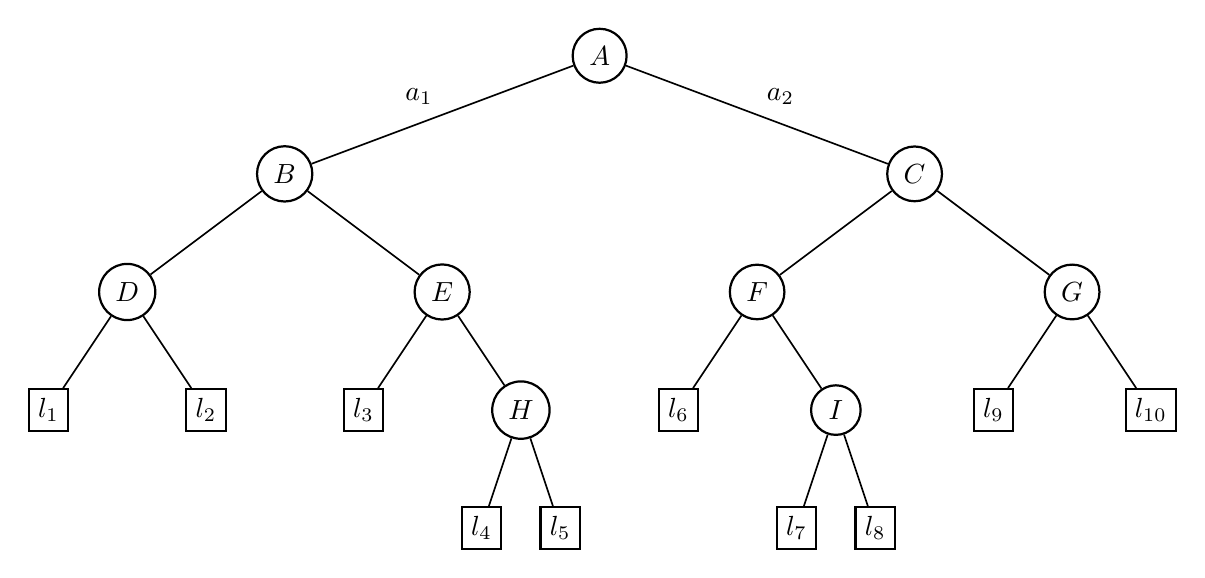
\begin{tikzpicture}[auto, semithick,
      every state/.style={draw=black, thick, fill=white, minimum size=5mm}]
    \node[state] at (0,0) (A) {$A$};
    \node[state] at (-4,-1.5) (B) {$B$};
    \node[state] at (4,-1.5) (C) {$C$};
    \node[state] at (-6,-3) (D) {$D$};
    \node[state] at (-2,-3) (E) {$E$};
    \node[state] at (2,-3) (F) {$F$};
    \node[state] at (6,-3) (G) {$G$};
    \node[state] at (-1,-4.5) (H) {$H$};
    \node[state] at (3,-4.5) (I) {$I$};
    \node[state, rectangle] at (-7,-4.5) (l1) {$l_1$};
    \node[state, rectangle] at (-5,-4.5) (l2) {$l_2$};
    \node[state, rectangle] at (-3,-4.5) (l3) {$l_3$};
    \node[state, rectangle] at (1,-4.5) (l6) {$l_6$};
    \node[state, rectangle] at (2.5,-6) (l7) {$l_7$};
    \node[state, rectangle] at (3.5,-6) (l8) {$l_8$};
    \node[state, rectangle] at (5,-4.5) (l9) {$l_9$};
    \node[state, rectangle] at (7,-4.5) (l10) {$l_{10}$};
    \node[state, rectangle] at (-1.5,-6) (l4) {$l_4$};
    \node[state, rectangle] at (-0.5,-6) (l5) {$l_5$};
    \path (A) edge node[above left] {$a_1$} (B);
    \path (A) edge node[above right] {$a_2$} (C);
    \path (B) edge (D); \path (B) edge (E);
    \path (C) edge (F); \path (C) edge (G);
    \path (D) edge (l1); \path (D) edge (l2);
    \path (E) edge (l3); \path (E) edge (H);
    \path (H) edge (l4); \path (H) edge (l5);
    \path (F) edge (l6); \path (F) edge (I);
    \path (I) edge (l7); \path (I) edge (l8);
    \path (G) edge (l9); \path (G) edge (l10);
  \end{tikzpicture}
\end{figure}
\begin{table}[H]
  \centering
  \begin{tabular}{|c|c|c|c|c|c|c|c|c|c|c|}
    \hline
    $l_i$ & 1 & 2 & 3 & 4 & 5 & 6 & 7 & 8 & 9 & 10 \\\hline
    $r_1$ & 1 & 2 & 3 & 3 & 5 & 0 & 2 & 3 & 2 & 4  \\\hline
  \end{tabular}
\end{table}

\begin{enumerate}
  \item Run the \textbf{minimax} algorithm and determine $v(A)$. Show all node values.

  \begin{solution}
    \begin{align*}
      v(D)&=\max(1,2)=2,\quad v(H)=\min(3,5)=3,\quad v(E)=\max(3,3)=3\\
      v(B)&=\min(2,3)=2\\
      v(I)&=\min(2,3)=2,\quad v(F)=\max(0,2)=2,\quad v(G)=\max(2,4)=4\\
      v(C)&=\min(2,4)=2\\
      v(A)&=\max(2,2)=\mathbf{2}
    \end{align*}
    Player 1 achieves value $2$; either action at $A$ is optimal.
  \end{solution}

  \item Apply $\alpha/\beta$-pruning (depth-first, left-to-right). Circle all pruned nodes/leaves and justify each cut.

  \begin{solution}
    Trace with $(\alpha,\beta)$ windows inherited from the parent:
    \begin{enumerate}
      \item Explore $B$ (min, $\beta=+\infty$, $\alpha=-\infty$). Explore $D$ (max): $l_1=1$ ($\alpha_D\to1$), $l_2=2$ ($\alpha_D\to2$). $v(D)=2$; $\beta_B\to2$.
      \item Explore $E$ (max, $\alpha=-\infty$, $\beta_B=2$): $l_3=3$, so $\alpha_E\to3\geq\beta_E=2$. \textbf{$\beta$-cut:} $H$ (and $l_4$, $l_5$) are \textbf{pruned}.
      \item $v(B)=\min(2,3)=2$. $\alpha_A\to2$.
      \item Explore $C$ (min, $\alpha_A=2$, $\beta=+\infty$). Explore $F$ (max, $\alpha=2$): $l_6=0$ (no change); explore $I$ (min, $\alpha=2$, $\beta=+\infty$): $l_7=2$, $\beta_I\to2\leq\alpha_I=2$. \textbf{$\alpha$-cut:} $l_8$ is \textbf{pruned}. $v(I)=2$, $v(F)=\max(0,2)=2$; $\beta_C\to2$.
      \item Explore $G$ (max, $\alpha=2$, $\beta_C=2$): $l_9=2$, $\alpha_G\to2$; $\beta_C=2\leq\alpha_G=2$. \textbf{$\alpha$-cut:} $l_{10}$ is \textbf{pruned}.
    \end{enumerate}
    \textbf{Pruned nodes/leaves:} $H,\; l_4,\; l_5,\; l_8,\; l_{10}$.
  \end{solution}
\end{enumerate}

\clearpage

%% ---- Q4: MCTS ----
\item \textit{Monte-Carlo Tree Search.}

\begin{enumerate}
  \item The partial MCTS tree below shows the state after 9 iterations (edge labels: $w/n$). The 10th selection phase follows path $\langle A, B, F \rangle$; node $I$ is expanded. The simulation runs 12 transitions from $I$ and the \textbf{reward to the last turn-taker is $-3$}.

  \begin{figure}[H]
    \centering
    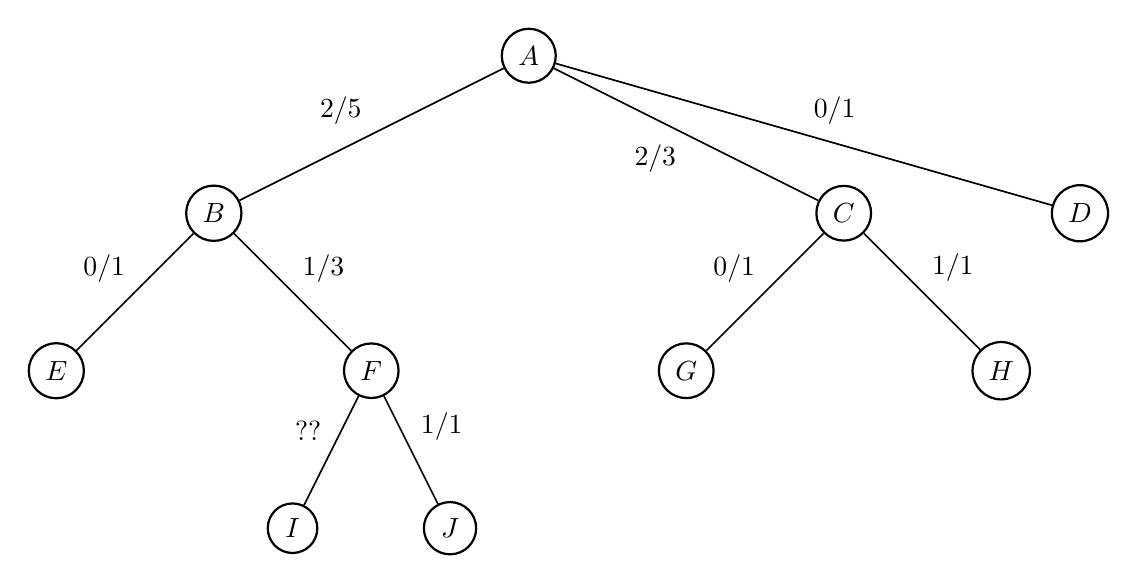
\begin{tikzpicture}[auto, semithick,
        every state/.style={draw=black, thick, fill=white, minimum size=5mm}]
      \node[state] at (0,0) (A) {$A$};
      \node[state] at (-4,-2) (B) {$B$};
      \node[state] at (4,-2) (C) {$C$};
      \node[state] at (7,-2) (D) {$D$};
      \node[state] at (-6,-4) (E) {$E$};
      \node[state] at (-2,-4) (F) {$F$};
      \node[state] at (2,-4) (G) {$G$};
      \node[state] at (6,-4) (H) {$H$};
      \node[state] at (-3,-6) (I) {$I$};
      \node[state] at (-1,-6) (J) {$J$};
      \path (A) edge node[midway, above left] {$2/5$} (B);
      \path (A) edge node[midway, below left] {$2/3$} (C);
      \path (A) edge node[midway, above right] {$0/1$} (D);
      \path (B) edge node[midway, above left] {$0/1$} (E);
      \path (B) edge node[midway, above right] {$1/3$} (F);
      \path (C) edge node[midway, above left] {$0/1$} (G);
      \path (C) edge node[midway, above right] {$1/1$} (H);
      \path (F) edge node[midway, above left] {$??$} (I);
      \path (F) edge node[midway, above right] {$1/1$} (J);
    \end{tikzpicture}
  \end{figure}

  Compute the updated Q-value estimates (show your work):
  \begin{enumerate}
    \item $q(A, \langle A,B\rangle)$
    \item $q(A, \langle A,C\rangle)$
    \item $q(F, \langle F,I\rangle)$
    \item $q(B, \langle B,F\rangle)$
  \end{enumerate}

  \begin{solution}
    $I$ is at depth 3 from root ($A$: depth 0). Simulation adds 12 transitions, so terminal depth $=15$ (odd $\Rightarrow$ Player 1 took the last action). Reward $-3$ is to Player 1 (a loss). Following the standard MCTS convention where $w$ counts wins for the player who \emph{moved into} that node: no win is recorded anywhere along the path.

    Updated counts on path $\{A\to B\to F\to I\}$:
    \begin{center}
    \begin{tabular}{lll}
      Edge $(A,B)$: & $w/n: 2/5 \to 2/6$ & (no win) \\
      Edge $(B,F)$: & $w/n: 1/3 \to 1/4$ & (no win) \\
      Edge $(F,I)$: & $w/n: \text{new} \to 0/1$ & (newly expanded)
    \end{tabular}
    \end{center}
    \begin{enumerate}
      \item $q(A,\langle A,B\rangle) = 2/6 \approx \mathbf{0.333}$
      \item $q(A,\langle A,C\rangle) = 2/3 \approx \mathbf{0.667}$ \quad (unchanged)
      \item $q(F,\langle F,I\rangle) = 0/1 = \mathbf{0}$
      \item $q(B,\langle B,F\rangle) = 1/4 = \mathbf{0.25}$
    \end{enumerate}
  \end{solution}

  \item The partial MCTS tree below shows the state after 35 iterations. Using the UCB formula with $c=\sqrt{2}$, determine which node is selected during the \textbf{36th selection phase}.

  \begin{figure}[H]
    \centering
    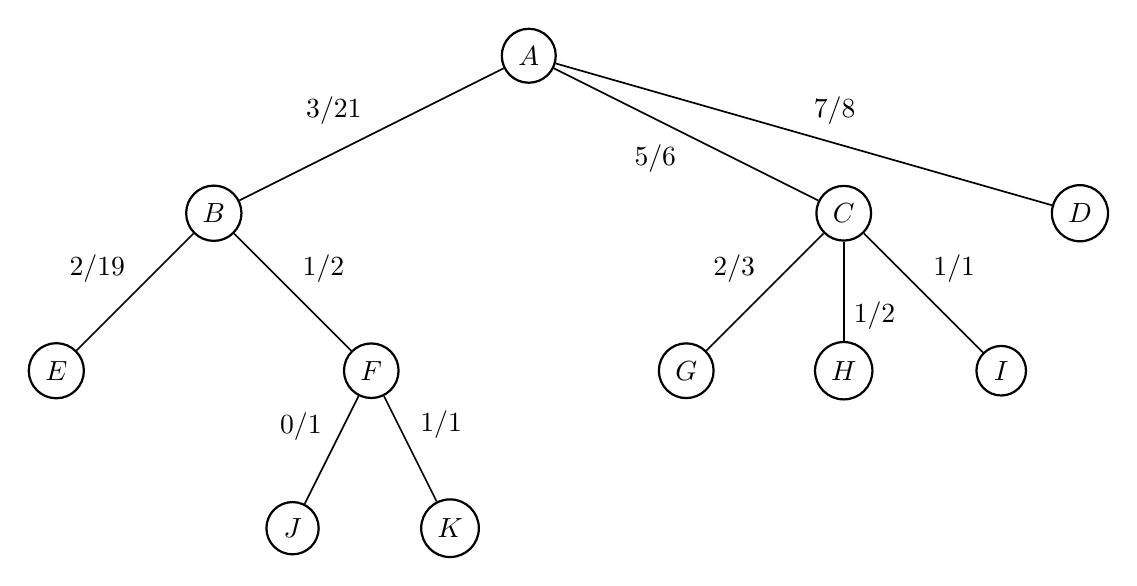
\begin{tikzpicture}[auto, semithick,
        every state/.style={draw=black, thick, fill=white, minimum size=5mm}]
      \node[state] at (0,0) (A) {$A$};
      \node[state] at (-4,-2) (B) {$B$};
      \node[state] at (4,-2) (C) {$C$};
      \node[state] at (7,-2) (D) {$D$};
      \node[state] at (-6,-4) (E) {$E$};
      \node[state] at (-2,-4) (F) {$F$};
      \node[state] at (2,-4) (G) {$G$};
      \node[state] at (4,-4) (Hh) {$H$};
      \node[state] at (6,-4) (Ii) {$I$};
      \node[state] at (-3,-6) (J) {$J$};
      \node[state] at (-1,-6) (K) {$K$};
      \path (A) edge node[midway, above left] {$3/21$} (B);
      \path (A) edge node[midway, below left] {$5/6$} (C);
      \path (A) edge node[midway, above right] {$7/8$} (D);
      \path (B) edge node[midway, above left] {$2/19$} (E);
      \path (B) edge node[midway, above right] {$1/2$} (F);
      \path (C) edge node[midway, above left] {$2/3$} (G);
      \path (C) edge node[midway, below right] {$1/2$} (Hh);
      \path (C) edge node[midway, above right] {$1/1$} (Ii);
      \path (F) edge node[midway, above left] {$0/1$} (J);
      \path (F) edge node[midway, above right] {$1/1$} (K);
    \end{tikzpicture}
  \end{figure}

  \begin{solution}
    $N(A)=35$. UCB scores from $A$ ($c=\sqrt{2}$, $\ln 35 \approx 3.555$):
    \begin{align*}
      \mathrm{UCB}(A,B)&=\tfrac{3}{21}+\sqrt{2}\sqrt{\tfrac{3.555}{21}}=0.143+0.581=0.724\\
      \mathrm{UCB}(A,C)&=\tfrac{5}{6}+\sqrt{2}\sqrt{\tfrac{3.555}{6}}=0.833+1.089=1.922\\
      \mathrm{UCB}(A,D)&=\tfrac{7}{8}+\sqrt{2}\sqrt{\tfrac{3.555}{8}}=0.875+0.943=1.818
    \end{align*}
    Select $C$ ($N(C)=6$, $\ln 6\approx1.792$):
    \begin{align*}
      \mathrm{UCB}(C,G)&=\tfrac{2}{3}+\sqrt{2}\sqrt{\tfrac{1.792}{3}}=0.667+1.093=1.760\\
      \mathrm{UCB}(C,H)&=\tfrac{1}{2}+\sqrt{2}\sqrt{\tfrac{1.792}{2}}=0.500+1.338=1.838\\
      \mathrm{UCB}(C,I)&=\tfrac{1}{1}+\sqrt{2}\sqrt{\tfrac{1.792}{1}}=1.000+1.893=2.893
    \end{align*}
    Select $I$. $I$ has no children $\Rightarrow$ \textbf{selection terminates at node $I$}.
  \end{solution}

\end{enumerate}

\clearpage

%% ============================================================
%%  SECTION 3: STOCHASTIC GAMES
%% ============================================================
\subsection*{Stochastic Games}

%% ---- Q5: Nash Value Iteration ----
\item \textit{Nash Value Iteration.}
Consider the Mammoth Herd stochastic game: states $\{\texttt{scarce}, \texttt{abundant}\}$, joint actions $\mathcal{A}=\{\texttt{e,e},\,\texttt{e,c},\,\texttt{c,e},\,\texttt{c,c}\}$. Rewards $r_1(s,a)$:
\begin{table}[H]
  \centering
  \begin{tabular}{|c|c|c|c|c|}
    \hline
    $s$ & \texttt{e,e} & \texttt{e,c} & \texttt{c,e} & \texttt{c,c} \\\hline
    \texttt{scarce}   & $2.0$ & $4.0$ & $0.0$ & $0.8$ \\\hline
    \texttt{abundant} & $2.5$ & $3.615$ & $0.0$ & $3.5$ \\\hline
  \end{tabular}
\end{table}
Rewards are symmetric: $r_2(s,(a_i,a_j))=r_1(s,(a_j,a_i))$. Transition probabilities $p(\texttt{abundant}\mid s,a)$:
\begin{table}[H]
  \centering
  \begin{tabular}{|c|c|c|c|c|}
    \hline
    $s$ & \texttt{e,e} & \texttt{e,c} & \texttt{c,e} & \texttt{c,c} \\\hline
    \texttt{scarce}   & $0.10$ & $0.40$ & $0.40$ & $0.60$ \\\hline
    \texttt{abundant} & $0.93$ & $0.90$ & $0.90$ & $0.95$ \\\hline
  \end{tabular}
\end{table}
Time horizon $T=2$, discount $\gamma=1.0$.

\begin{enumerate}
  \item \textbf{Initialize} ($t=1$): Compute $q_i^*(s,a;1)=r_i(s,a)$ for all $s,a,i$.

  \begin{solution}
    $q_1^*(s,a;1)$ equals the reward table above. By symmetry, $q_2^*(s,a;1)=q_1^*(s,\mathrm{swap}(a);1)$, e.g.\ $q_2^*(\texttt{scarce},\texttt{e,c};1)=r_1(\texttt{scarce},\texttt{c,e})=0.0$.
  \end{solution}

  \item \textbf{Stage games at $t=1$}: For each state find the symmetric pure Nash equilibrium and compute $v_i^*(s;1)$.

  \begin{solution}
    \textbf{Scarce.}
    \begin{center}\begin{tabular}{|c|c|c|}\hline & \texttt{e} & \texttt{c}\\\hline \texttt{e} & $(2.0,2.0)$ & $(4.0,0.0)$\\\hline \texttt{c} & $(0.0,4.0)$ & $(0.8,0.8)$\\\hline\end{tabular}\end{center}
    $\mathrm{BR}_1(\texttt{e})=\texttt{e}$ (since $2.0>0.0$). \textbf{NE: \texttt{e,e}.} $v_i^*(\texttt{scarce};1)=2.0$.

    \textbf{Abundant.}
    \begin{center}\begin{tabular}{|c|c|c|}\hline & \texttt{e} & \texttt{c}\\\hline \texttt{e} & $(2.5,2.5)$ & $(3.615,0.0)$\\\hline \texttt{c} & $(0.0,3.615)$ & $(3.5,3.5)$\\\hline\end{tabular}\end{center}
    $\mathrm{BR}_1(\texttt{e})=\texttt{e}$; check \texttt{c,c}: $\mathrm{BR}_1(\texttt{c})=\texttt{e}$ ($3.615>3.5$). \textbf{NE: \texttt{e,e}.} $v_i^*(\texttt{abundant};1)=2.5$.
  \end{solution}

  \item \textbf{Back up to $t=0$}: Compute $q_i^*(s,a;0)=r_i(s,a)+\gamma\sum_{s'}p(s'\mid s,a)\,v_i^*(s';1)$.

  \begin{solution}
    With $v_1^*(\texttt{sc};1)=2.0$, $v_1^*(\texttt{ab};1)=2.5$, $\gamma=1$: contribution from future $= 2.0 + 0.5\,p(\texttt{ab}\mid s,a)$.

    \textbf{Scarce} ($\rho=p(\texttt{ab}\mid\texttt{sc},a)$):
    \begin{align*}
      \texttt{e,e}&: 2.0+2.0+0.5(0.10)=4.05 & \texttt{e,c}&: 4.0+2.0+0.5(0.40)=6.20\\
      \texttt{c,e}&: 0.0+2.0+0.5(0.40)=2.20 & \texttt{c,c}&: 0.8+2.0+0.5(0.60)=3.10
    \end{align*}
    \textbf{Abundant} ($\rho'=p(\texttt{ab}\mid\texttt{ab},a)$):
    \begin{align*}
      \texttt{e,e}&: 2.5+2.0+0.5(0.93)=4.965 & \texttt{e,c}&: 3.615+2.0+0.5(0.90)=6.065\\
      \texttt{c,e}&: 0.0+2.0+0.5(0.90)=2.450 & \texttt{c,c}&: 3.5+2.0+0.5(0.95)=5.975
    \end{align*}
  \end{solution}

  \item \textbf{Stage games at $t=0$}: Find the symmetric pure NE using $q_i^*(\cdot,\cdot;0)$.

  \begin{solution}
    \textbf{Scarce:} $\mathrm{BR}_1(\texttt{e})=\texttt{e}$ ($4.05>2.20$); check \texttt{c,c}: $\mathrm{BR}_1(\texttt{c})=\texttt{e}$ ($6.20>3.10$). \textbf{NE: \texttt{e,e}} ($v=4.05$).

    \textbf{Abundant:} $\mathrm{BR}_1(\texttt{e})=\texttt{e}$ ($4.965>2.450$); check \texttt{c,c}: $\mathrm{BR}_1(\texttt{c})=\texttt{e}$ ($6.065>5.975$). \textbf{NE: \texttt{e,e}} ($v=4.965$).
  \end{solution}

  \item Compare equilibria at $t=0$ and $t=1$. Does the equilibrium action change?

  \begin{solution}
    The equilibrium is \texttt{e,e} in both states at both time steps. It does not change. Intuitively, the immediate temptation to exploit (\texttt{e,c} yields $4.0 > 0.8$) dominates regardless of future state values, because neither agent can unilaterally benefit from switching to \texttt{c}. A longer horizon or stronger future consequences (larger $\gamma$ with a payoff structure favoring \texttt{c,c} more heavily) would be needed to shift the equilibrium.
  \end{solution}
\end{enumerate}

\clearpage

%% ---- Q6: Nash Q-Learning ----
\item \textit{Nash Q-Learning.}
Agents learn the Mammoth Herd game using Nash Q-learning ($\alpha=0.5$, $\gamma=1.0$). Current estimates $\tilde{q}_1(s,a)$ (with $\tilde{q}_2$ symmetric):
\begin{table}[H]
  \centering
  \begin{tabular}{|c|c|c|c|c|}
    \hline
    $s$ & \texttt{e,e} & \texttt{e,c} & \texttt{c,e} & \texttt{c,c} \\\hline
    \texttt{scarce}   & $2.0$ & $3.8$ & $0.2$ & $1.5$ \\\hline
    \texttt{abundant} & $3.0$ & $4.1$ & $0.3$ & $4.0$ \\\hline
  \end{tabular}
\end{table}
Current state: $\texttt{scarce}$. Joint action: $\texttt{e,c}$. Rewards: $r_1'=4.0$, $r_2'=0.0$. Next state: $\texttt{abundant}$.

\begin{enumerate}
  \item Find the symmetric Nash equilibrium of the \texttt{abundant} stage game and compute $\tilde{v}_1(\texttt{abundant})$.

  \begin{solution}
    \begin{center}\begin{tabular}{|c|c|c|}\hline & \texttt{e} & \texttt{c}\\\hline \texttt{e} & $(3.0,3.0)$ & $(4.1,0.3)$\\\hline \texttt{c} & $(0.3,4.1)$ & $(4.0,4.0)$\\\hline\end{tabular}\end{center}
    Check \texttt{e,e}: $\mathrm{BR}_1(\texttt{e})=\texttt{e}$ ($3.0>0.3$). \textbf{NE: \texttt{e,e}.} $\tilde{v}_1(\texttt{abundant})=3.0$.

    (Check \texttt{c,c}: $\mathrm{BR}_1(\texttt{c})=\texttt{e}$ ($4.1>4.0$). Not a NE.)
  \end{solution}

  \item Update $\tilde{q}_1(\texttt{scarce},\texttt{e,c})$.

  \begin{solution}
    \[\tilde{q}_1 \leftarrow (1-0.5)(3.8)+0.5(4.0+1.0\cdot3.0)=1.9+3.5=\mathbf{5.4}\]
  \end{solution}

  \item Update $\tilde{q}_2(\texttt{scarce},\texttt{e,c})$.

  \begin{solution}
    By symmetry $\tilde{v}_2(\texttt{abundant})=3.0$. $r_2'=0.0$.
    \[\tilde{q}_2 \leftarrow (1-0.5)(0.0)+0.5(0.0+1.0\cdot3.0)=0+1.5=\mathbf{1.5}\]
  \end{solution}

  \item After the update, does the symmetric NE of the \texttt{scarce} stage game change?

  \begin{solution}
    Updated $\tilde{q}_1(\texttt{scarce},\cdot)$: \texttt{e,e}$=2.0$, \texttt{e,c}$=5.4$, \texttt{c,e}$=0.2$, \texttt{c,c}$=1.5$.
    $\mathrm{BR}_1(\texttt{e})=\texttt{e}$ ($2.0>0.2$). \textbf{NE remains \texttt{e,e}.} No change.
  \end{solution}

  \item Briefly describe the \textbf{equilibrium selection problem} in Nash Q-learning.

  \begin{solution}
    When a stage game has multiple Nash equilibria, agents must agree on which NE to use when computing $\tilde{v}_i(s)$ for the update step. If agents independently select different equilibria, the updates become inconsistent and the algorithm may fail to converge. This is a fundamental limitation of Nash Q-learning compared to single-agent Q-learning, where the max operator uniquely selects the best action.
  \end{solution}
\end{enumerate}

\end{enumerate}
\end{document}